\documentclass[c,unicode,russian]{beamer}
\usepackage{hyperref}
\usepackage{alltt}
\usepackage{verbatim}
\usepackage{fancyvrb}

\usepackage{fontspec}
\setsansfont{Ubuntu}
\setmonofont{Ubuntu Mono}
\usepackage{polyglossia}
\setdefaultlanguage{russian}

\useinnertheme{metropolis}
\useoutertheme{metropolis}
\usecolortheme{metropolis}

\usepackage{listings,xcolor}
\usepackage{../../listings-golang/listings-golang}   % Golang
\lstset{%
    keywordstyle=\color{blue},
    commentstyle=\color[rgb]{0.13,0.54,0.13},
    backgroundcolor=\color{yellow!10},
    basicstyle=\small\tt,
    stringstyle=\color{red}\ttfamily,
    showstringspaces=false,
    belowcaptionskip=-1pt,
    xleftmargin=-15pt,
    framexleftmargin=-15pt,
    framexrightmargin=5pt,
    framextopmargin=5pt,
    framexbottommargin=5pt,
    framesep=0pt,
    rulesep=0pt
}
\lstdefinestyle{cpp}{%
    language=C++,
    morecomment=[l][\color{magenta}]{\#}
}
\lstdefinestyle{python}{%
    language=Python
}
\lstdefinestyle{php}{%
    language=php
}
\lstdefinestyle{html}{%
    language=html
}
\lstdefinestyle{go}{% add your own preferences
    language=Golang
}

\usepackage{caption}
\renewcommand{\lstlistingname}{Код} % Listing -> Algorithm
\DeclareCaptionFont{white}{\color{white}}
\DeclareCaptionFormat{listing}{\colorbox{gray}{\parbox{\textwidth}{#1#2#3}}}
\captionsetup[lstlisting]{format=listing,labelfont=white,textfont=white}

% logo of my university
\titlegraphic{\vspace{-35pt}\hspace{-1cm}\includegraphics[width=\paperwidth]{../../_static/logo.png}}

\date{}
\author{Основы Веб-программирования}
\institute{Кафедра Интеллектуальных Информационных Технологий, ИнФО, УрФУ}

\usepackage{array}      % Table

\title{Веб-сервер}

\begin{document}

% Slide #1
\frame{\titlepage}

% Slide #2
\begin{frame}{Ресурсы}
    \url{https://ru.wikipedia.org/wiki/Веб-сервер}\newline
    \url{http://lectureswww.readthedocs.org/5.web.server/index.html}
\end{frame}

% Slide #3
\begin{frame}{Называют}

    \begin{itemize}
        \item Железо, на котором запущенны сервисы и есть подключение с сети.
        \item Программу, которая слушает 80 порт и отвечает на HTTP запросы
    \end{itemize}

    \begin{center}
        \includegraphics[width=4.2in]{media/web-server.png}
    \end{center}

\end{frame}

% Slide #4
\begin{frame}{Типы HTTP серверов}
    \begin{itemize}
        \item \textbf{Статический веб-сервер}, или стек, посылает размещенные
            на нем файлы в браузер “как есть”. (nginx, Apache)

        \item \textbf{Динамических веб-сервер} состоит из статического
            веб-сервера плюс дополнительного программного обеспечения, наиболее
            часто \textbf{сервером приложений} и базы данных.
            (Gunicorn, Waitress, Tornado)
    \end{itemize}
\end{frame}

% Slide #5
\begin{frame}{Типы сайтов}
    \begin{itemize}
        \item Статические Веб-сайты проще всего установить. К ним относятся
            HTML страницы, картинки, шрифты, CSS стили и прочее\ldots
        \item Динамический Веб-сайт означает, что сервер обрабатывает данные или даже
            генерирует их на лету из базы данных. Это обеспечивает больше
            гибкости, но технически сложнее в обслуживании, что делает его
            более сложным в разработке.

    \end{itemize}
\end{frame}

% Slide #6
\begin{frame}{Связь Веб-приложения с HTTP-сервером}
    \begin{itemize}
        \item CGI
        \item FastCGI
        \item Встроенный сервер
        \item WSGI
    \end{itemize}
\end{frame}

% Slide #7
\begin{frame}{CGI}
    \begin{center}
        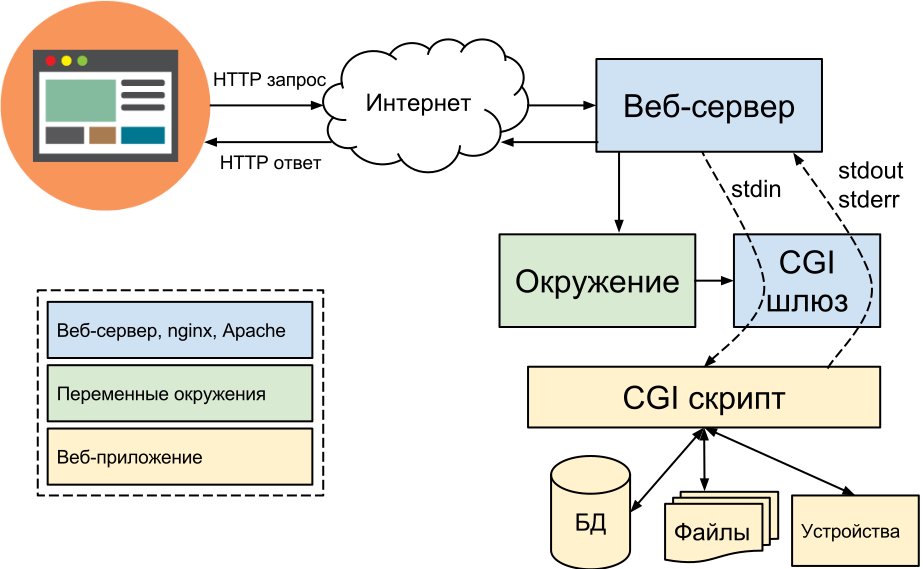
\includegraphics[width=4.2in]{media/cgi.png}
    \end{center}
\end{frame}

% Slide #8
\begin{frame}{CGI}
    CGI — это не язык программирования!\newline
    Это простой протокол, позволяющий Веб-серверу передавать данные через
    \textbf{stdin} и читать их из \textbf{stdout}. \newline\newline
    Поэтому, в качестве CGI-обработчика может использоваться
    программа на любом языке, способном работать со стандартными потоками
    ввода-вывода.
\end{frame}

% Slide #9
\begin{frame}{CGI. Самый простой сервер.}
    python3 -m http.server --cgi 8000
\end{frame}

% Slide #10
\begin{frame}[fragile]{CGI\@. Hello World!}

    \begin{lstlisting}[style=cpp, caption=Си]
    #include <stdio.h>
    int main(void) {
      printf("Content-Type: text/plain\n\n");
      printf("Hello, world!\n\n");
      return 0;
    }
    \end{lstlisting}

    \begin{lstlisting}[style=python, caption=Python]
    #!/usr/bin/python
    print("Content-Type: text/plain\n\nHello, world!")
    \end{lstlisting}
\end{frame}

% Slide #11
\begin{frame}[fragile]{CGI\@. Переменные окружения}

    \begin{lstlisting}[style=python, caption=Python]
    #!/usr/bin/python
    import os

    print("Content-type: text/html\r\n\r\n")
    print("<font size=+10>Environment</font><br>")

    for param in os.environ.keys():
        print("<b>%20s</b>: %s<br>" %
              (param, os.environ[param]))
    \end{lstlisting}
\end{frame}

% Slide #12
\begin{frame}[fragile]{CGI\@. Переменные окружения}
    \begin{center}
        \includegraphics[width=4.2in]{media/cgi_env.png}
    \end{center}
\end{frame}

% Slide #13
\begin{frame}{CGI\@. Преимущества}
    \begin{itemize}
        \item Процесс CGI скрипта не зависит от Веб-сервера и в случае падения
            ни как не отразится на работе последнего.
        \item Может быть написан на любом языке программирования.
        \item Поддерживается большинством Веб-серверов.
    \end{itemize}
\end{frame}

% Slide #14
\begin{frame}[fragile]{CGI\@. Недостатки}
    \textbf{Потребление ресурсов}\newline

    Дело в том, что каждое обращение к CGI-приложению вызывает порождение
    нового процесса, со всеми вытекающими отсюда накладными расходами.
\end{frame}

% Slide #15
\begin{frame}{FastCGI}
    \begin{center}
        \includegraphics[width=4.2in]{media/fastcgi.png}
    \end{center}
\end{frame}

% Slide #16
\begin{frame}{FastCGI}
    \begin{itemize}
        \item В отличие от CGI, FastCGI использует постоянно запущенные
            процессы для обработки множества запросов.
        \item FastCGI-процессы используют для связи с сервером \textbf{Unix Domain
            Sockets} или \textbf{TCP/IP}.
    \end{itemize}
\end{frame}

% Slide #17
\begin{frame}[fragile]{FastCGI. Приложение}
    \textbf{Сборка}: gсс -o hello.fcgi hello.cpp -lfcgi\newline
    \textbf{Запуск}: spawn-fcgi -p 5000 -n hello.fcgi

    \begin{lstlisting}[style=cpp, caption=Си]
    #include "fcgi_stdio.h"
    #include <stdlib.h>

    int main(void)
    {
     while(FCGI_Accept() >= 0)
     {
         printf("Content-type: text/html\r\n"
                "Status: 200 OK\r\n\r\nHello World!");
     }
     return 0;
    }
    \end{lstlisting}
\end{frame}

% Slide #18
\begin{frame}{Встроенный сервер}
    В некоторых языках, например Go, уже существует встроенный
    Веб-сервер.

    \begin{center}
        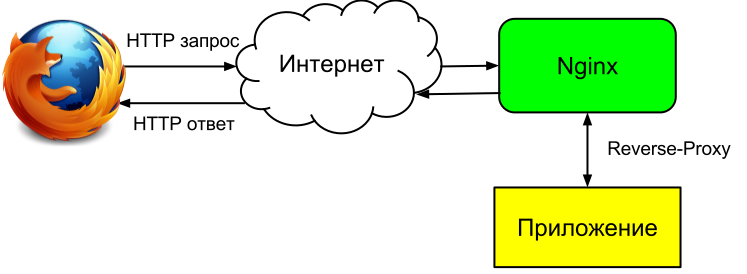
\includegraphics[width=4.2in]{media/reverse_proxy.png}
    \end{center}
\end{frame}

% Slide #19
\begin{frame}[fragile]{Встроенный сервер. FastCGI}
    В этом случае не нужно запускать отдельно fcgi сервер, например
    spawn-fcgi.

    \begin{lstlisting}[style=go, caption=Go]
    package main
    import (
        "fmt"
        "net"
        "net/http"
        "net/http/fcgi"
    )

    func handler(res http.ResponseWriter,
                 req *http.Request) {
        fmt.Fprint(res, "Hello World!")
    }
    \end{lstlisting}
\end{frame}

% Slide #20
\begin{frame}[fragile]{Встроенный сервер. FastCGI}
    go run hello.go
    \begin{lstlisting}[style=go, caption=Go]
    func main() {
        // For local machine
        // l, _ := net.Listen("unix",
        //                    "/var/run/go-fcgi.sock")

        // TCP 5000 listen
        l, err := net.Listen("tcp", "0.0.0.0:5000")
        if err != nil {
            return
        }
        http.HandleFunc("/", handler)
        fcgi.Serve(l, nil)
    }
    \end{lstlisting}
\end{frame}

% Slide #21
\begin{frame}[fragile]{Встроенный сервер. HTTP}
    Может запускаться самостоятельно без дополнительных программ и
    настроек.

    \begin{lstlisting}[style=go, caption=Go]
    package main

    import (
        "fmt"
        "net/http"
    )

    func handler(w http.ResponseWriter,
                 r *http.Request) {
        fmt.Fprintln(w, "Hello World!")
    }
    \end{lstlisting}
\end{frame}

% Slide #22
\begin{frame}[fragile]{Встроенный сервер. HTTP}
    go run hello.go
    \begin{lstlisting}[style=go, caption=Go]
    func main() {
        http.HandleFunc("/", handler)
        http.ListenAndServe(":8000", nil)
    }
    \end{lstlisting}
\end{frame}

% Slide #23
\begin{frame}{WSGI. PEP-333. PEP-3333}
    \textbf{WSGI} предоставляет простой и универсальный интерфейс
    для соединения веб-серверов, веб-приложений и прослоек между ними.

    \begin{itemize}
        \item Application
        \item Server
        \item Middleware
    \end{itemize}

    Все Python фреймворки поддерживают WSGI.\newline Даже Django!


\end{frame}

\end{document}
